\documentclass[aspectratio=169]{beamer}

\usepackage{microtype}
\usepackage{tikzpeople}
\usepackage{drawstack}
\usepackage{graphicx}
\usepackage{fontawesome}
\usepackage{multirow}
\usepackage{fancyvrb}
\usepackage{listings}
\usepackage{siunitx}
\usepackage{tikz}
\usetikzlibrary{calc}
\usetikzlibrary{arrows.meta}
\usetikzlibrary{positioning}
\tikzstyle{block} = [draw, rectangle, 
    minimum height=2em, minimum width=2em]

\newcommand{\cipher}[1]{\texttt{#1}}
\newcommand\presdate{June 18, 2020}

\setbeamercovered{transparent}

\usetheme[]{metropolis}
\metroset{block=fill}

\title{Android: Notifier (Server)}
\date{\presdate}

\author{Marcel Nageler, Sebastian Knoll, Martin Unterguggenberger}
\institute{}

\setbeamertemplate{frame footer}{Android: Notifier (Server) --- Graz, \presdate}

\definecolor{links}{HTML}{2A1B81}
\hypersetup{colorlinks,linkcolor=,urlcolor=links}

\begin{document}
  \maketitle

  %\begin{frame}
  %  \begin{figure}
  %    \centering
  %    \includegraphics[width=\textwidth]{figures/...}
  %    %\caption{}
  %  \end{figure}
  %\end{frame}

\section{Introduction}
  \begin{frame}{Motivation}
    \begin{itemize}
      \item Sending notifications from a phone to a PC
      \pause
      \item We do not trust the server
    \end{itemize}
  \end{frame}

  \begin{frame}{Security Goals}
    \begin{itemize}
      \item \textbf{Confidentialty}
        \setbeamercovered{invisible}
        \onslide<1>{$\rightarrow$ Third parties cannot read any messages}
        \setbeamercovered{transparent}
      \pause
      \item \textbf{Integrity}
        \setbeamercovered{invisible}
        \onslide<2>{$\rightarrow$ Third parties cannot alter or forge messages}
        \setbeamercovered{transparent}
      \pause
      % \item \textbf{Availability}
      %   \setbeamercovered{invisible}
      %   \onslide<3>{$\rightarrow$ Timely and reliable access to the information}
      %   \setbeamercovered{transparent}
      % \pause
      \item \textbf{Authencity}
        \setbeamercovered{invisible}
        \onslide<3>{$\rightarrow$ The sender is who they claim to be}
        \setbeamercovered{transparent}
      \pause
      \item \textbf{Forward Secrecy}
        \setbeamercovered{invisible}
        \onslide<4>{$\rightarrow$ Leak of a private key does not affect past communication}
        \setbeamercovered{transparent}
      \pause
      \item \textbf{Identity Hiding}
        \setbeamercovered{invisible}
        \onslide<5>{$\rightarrow$ Third parties do not see the public key of the sender}
        \setbeamercovered{transparent}
    \end{itemize}
  \end{frame}

\section{Implementation}

  \begin{frame}{Implementation}
    \begin{figure}
      \centering
      \only<1|handout:0>{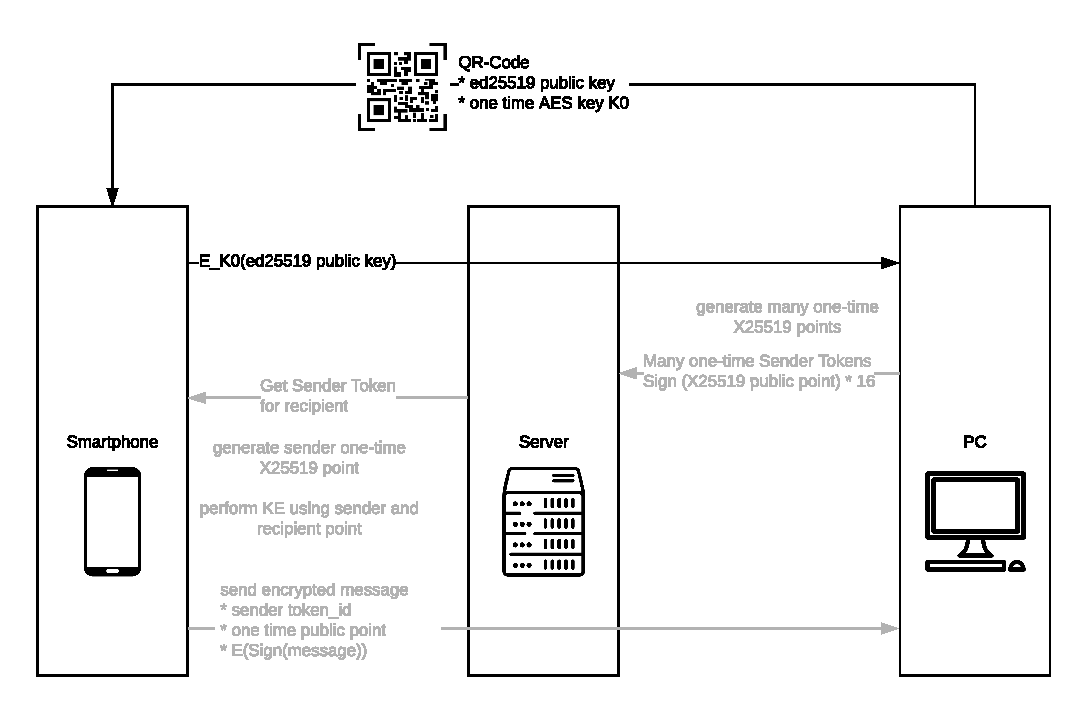
\includegraphics[width=0.7\textwidth]{figures/anim1}}%
      \only<2|handout:0>{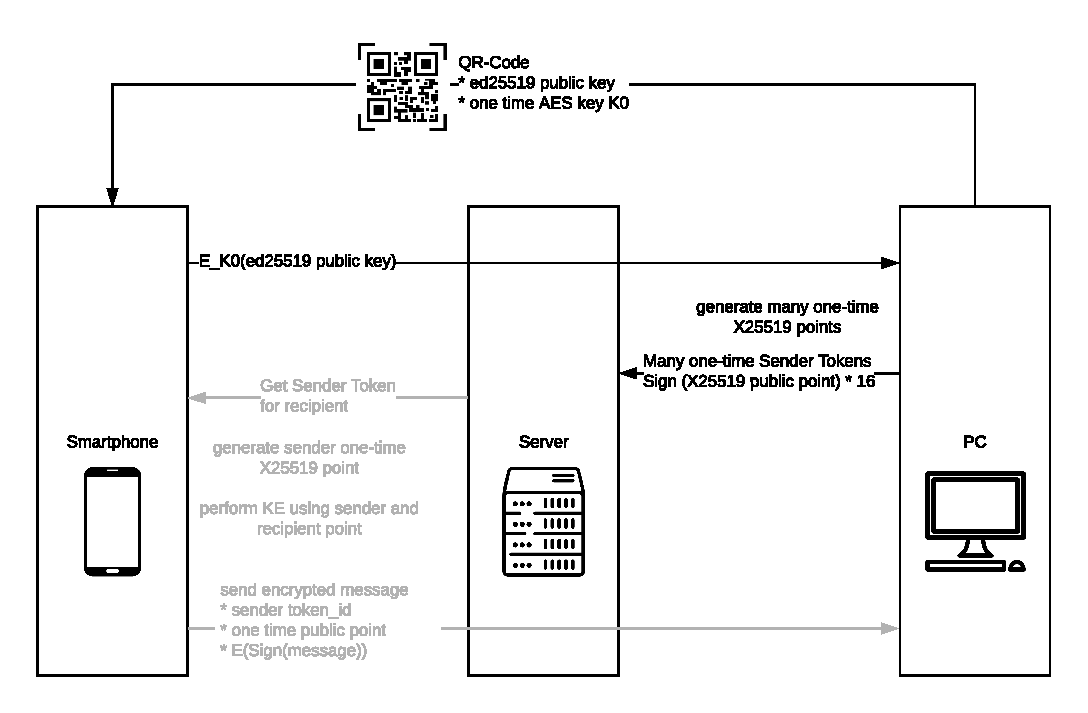
\includegraphics[width=0.7\textwidth]{figures/anim2}}%
      \only<3>{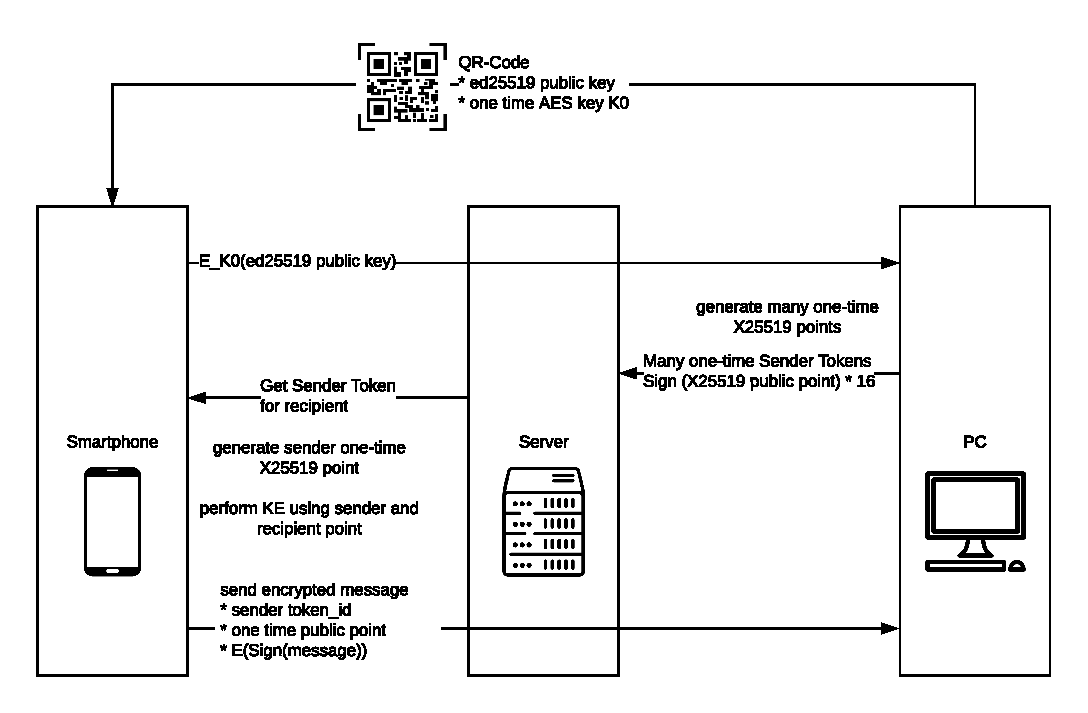
\includegraphics[width=0.7\textwidth]{figures/anim3}}%
      %\caption{}
    \end{figure}
  \end{frame}

  \begin{frame}{Implementation (cont.)}
    \begin{itemize}
      \item Server $\leftrightarrow$ PC
      \begin{itemize}
        \item Websockets for realtime communication
      \end{itemize}
      \item Server $\leftrightarrow$ smartphone
      \begin{itemize}
        \item Certificate Pinning
        \item plain \texttt{GET} and \texttt{POST} requests
      \end{itemize}
    \end{itemize}
  \end{frame}

  \begin{frame}{Curve25519}
    Popularity increased considerably after 2013 when it was discovered that the NSA had potentially implemented a backdoor into Dual\_EC\_DRBG
    \begin{itemize}
      \item Curve25519 implemented in Go standard library
      \item Server and Client written in Go
      \item Android application uses Bouncy Castle library
    \end{itemize}
  \end{frame}

  \begin{frame}{Asymmetric cryptography}
    \cipher{Curve25519} is designed for use with the elliptic curve Diffie–Hellman (ECDH)
    \begin{itemize}
      \item Digital Signature Algorithm \cipher{Ed25519}
      \item Key Exchange Algorithm \cipher{X25519}
      \item Shared \cipher{AES-256-GCM} key for message encryption
    \end{itemize}
  \end{frame}

  \begin{frame}{Android Keystore}
    Store cryptographic keys in a container to make it more difficult to extract from the device
    \begin{itemize}
      \item Key material remaining non-exportable
      \item Android Keystore System does not support \cipher{Curve25519}
      \item Asymmetric keys stored in encrypted file
      \item Android Keystore \cipher{AES-128-GCM} to encrypt file
    \end{itemize}
  \end{frame}

  \begin{frame}{Live Demo}
    \centering
    You've been watching it the whole time
    \begin{figure}
      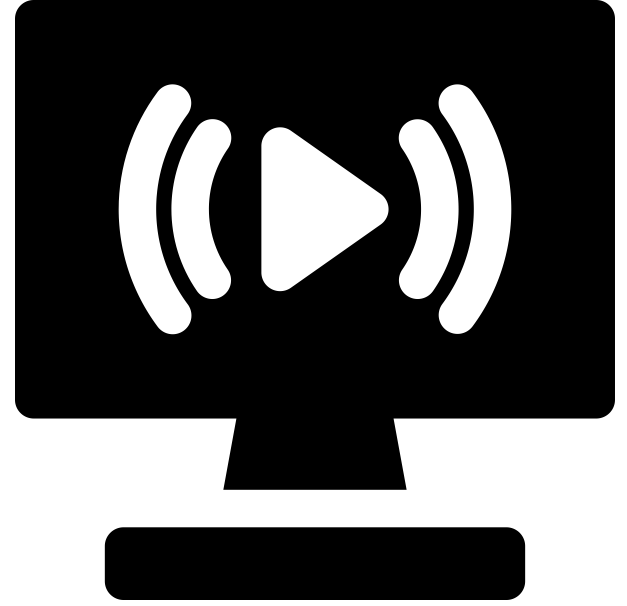
\includegraphics[width=0.3\textwidth]{figures/live}
    \end{figure}
  \end{frame}

  \maketitle
%  \nocite{*}
%  \begin{frame}{References}
%    %\printbibliography
%    \bibliographystyle{alpha}
%    \bibliography{references}
%  \end{frame}
\end{document}
